\subsection{Decision Model과 Cross-Encoder의 재정렬 성능 비교 (RQ2)}

\label{sec:ch4_3}

최종 선택 이전의 상위 10개 후보를 비교하여 재정렬 단계의 성능을 살펴보았다. 공통 BM25 후보 합집합의 문항별 평균 gold Recall은 77.21\%였다. 재정렬 후 shortlist 합집합의 Recall은 CE 69.47\%, Jev 74.63\%로 Jev가 5.16\%p 높았다. 모든 gold가 shortlist에 남은 문항도 112개(49.56\%)에서 130개(57.52\%)로 증가하였다(그림 2). 이 수치는 최종 선택 성능과 구별되는 후보 유지 수준이다.

\begin{figure}[H]
\centering
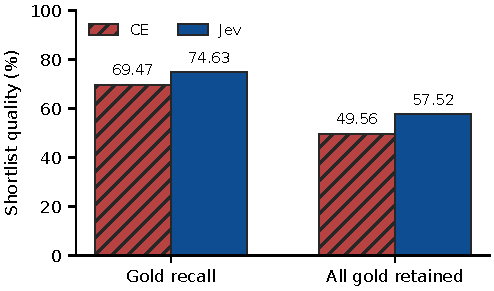
\includegraphics[width=\linewidth]{research/chapter4/figures/section-figures-v1/fig_4_3_shortlist_quality_column.pdf}
\caption{상위 후보 합집합의 정답 근거 유지 수준(226문항). Recall은 문항별 평균이며 오차막대는 산출하지 않았다.}
\label{fig:ch4_3}
\end{figure}

후보 유지 수준의 개선이 최종 완전 회수로 모두 이어지지는 않았다. 각 후보 목록에서 하나만 선택하는 제약을 반영하면, shortlist에서 모든 gold를 동시에 선택할 수 있는 문항은 CE 104개, Jev 120개로 줄어든다. 실제 완전 회수는 각각 77개와 79개였다. 따라서 Jev는 상위 후보에서 정답 근거를 더 많이 유지했지만, 후속 선택과 목록 구조의 제약이 남았다. 이 단계의 비교는 관련성 분류 정확도나 최종 답변 정확도와 구별된다. RQ2 중 지연시간 비교는 본 결과 보고의 범위에 포함하지 않았다.
